\documentclass[aspectratio=169,9pt]{beamer}

% ===== Speaker Notes (toggle: uncomment next 2 lines to enable) =====
% \usepackage{pgfpages}
% \setbeameroption{show notes on second screen=right}

% ===== Chinese font support for speaker notes =====
\usepackage{xeCJK}
\setCJKmainfont{STSong}
\setCJKsansfont{Heiti SC}

% ===== Compile with: xelatex presentation.tex =====
\usepackage{fontawesome5}
\usepackage{graphicx}
\usepackage{tikz}
\usepackage{booktabs}
\usepackage{array}
\usetikzlibrary{positioning}

% ===== Theme =====
\usetheme{Madrid}
\usecolortheme{seahorse}
\setbeamertemplate{navigation symbols}{}
\setbeamertemplate{itemize items}[circle]
\setlength{\leftmargini}{1em}
\setlength{\leftmarginii}{1em}

% ===== Colors =====
\definecolor{sjtuBlue}{RGB}{17,74,121}
\definecolor{sjtuLightBlue}{RGB}{0,113,188}
\definecolor{accentGold}{RGB}{180,140,50}
\definecolor{lightBg}{RGB}{245,248,252}

\setbeamercolor{palette primary}{bg=sjtuBlue,fg=white}
\setbeamercolor{palette secondary}{bg=sjtuLightBlue,fg=white}
\setbeamercolor{palette tertiary}{bg=sjtuBlue,fg=white}
\setbeamercolor{structure}{fg=sjtuBlue}
\setbeamercolor{title}{fg=sjtuBlue}
\setbeamercolor{block title}{bg=sjtuBlue,fg=white}
\setbeamercolor{block body}{bg=lightBg}
\setbeamercolor{item}{fg=sjtuBlue}

\setbeamerfont{title}{size=\Large,series=\bfseries}
\setbeamerfont{frametitle}{size=\large,series=\bfseries}

% ===== Utility Commands =====
\newcommand{\highlight}[1]{\textcolor{sjtuBlue}{\textbf{#1}}}
\newcommand{\metric}[1]{\colorbox{accentGold!20}{\textcolor{sjtuBlue}{\textbf{#1}}}}
\newcommand{\tagitem}[1]{\colorbox{sjtuBlue!15}{\small\textcolor{sjtuBlue}{#1}}}

% ============================================================
% === EDIT ZONE: Global Metadata (modify these variables) ===
% ============================================================
\newcommand{\PresenterName}{Xinchen Li}
\newcommand{\PresentationTitle}{Your Presentation Title Here}
\newcommand{\PresentationSubtitle}{Ph.D. Candidate | High Energy Physics \& HPC}
\newcommand{\Affiliation}{Shanghai Jiao Tong University \textperiodcentered{} Tsung-Dao Lee Institute}
\newcommand{\PresentationDate}{March 12, 2026}
\newcommand{\Email}{starleetdli@gmail.com}
\newcommand{\Phone}{13153522674}
\newcommand{\GitHub}{StarLee2}

% === EDIT: Show photo on cover page? (true/false) ===
\newif\ifShowPhoto
\ShowPhototrue   % Change to \ShowPhotofalse to hide photo

% === EDIT: Cover page summary lines ===
\newcommand{\CoverLineOne}{Your first summary line about research background}
\newcommand{\CoverLineTwo}{Your second summary line about methods or systems}
\newcommand{\CoverLineThree}{Your third summary line about outcomes or impact}
% ============================================================

% ===== pgfpages-compatible Header/Footer/Frametitle =====
\makeatletter

% --- Headline: header image on content pages, skip on plain ---
\setbeamertemplate{headline}{%
  \ifbeamer@plainframe\else
    \vbox to 0pt{%
      \vss
      \hbox to \paperwidth{%
        \hss
\includegraphics[width=\paperwidth]{assets/页眉newstyle.png}\hss
      }%
    }%
    \vspace{0.93cm}%
  \fi
}

% --- Footline: footer image on content pages, skip on plain ---
\setbeamertemplate{footline}{%
  \ifbeamer@plainframe\else
    \vbox to 0.71cm{%
      \vfill
      \hbox to \paperwidth{%
        \hss
\includegraphics[width=\paperwidth]{assets/页脚.png}\hss
      }%
    }%
  \fi
}

% --- Frametitle: white text overlaid on header image ---
\setbeamertemplate{frametitle}{%
  \ifbeamer@plainframe\else
    \vspace{-0.75cm}%
    \hspace{0.45cm}%
    \usebeamerfont{frametitle}\textcolor{white}{\insertframetitle}%
    \vspace{0.15cm}%
  \fi
}

\makeatother

\title{\PresentationTitle}
\subtitle{\PresentationSubtitle}
\author{\PresenterName}
\institute{\Affiliation}
\date{\PresentationDate}

\begin{document}

% ==================== Cover Page (Fixed Layout) ====================
% --- Cover WITH photo ---
\ifShowPhoto
\begin{frame}[plain]
\begin{tikzpicture}[remember picture,overlay]
    \node[anchor=center,inner sep=0pt] at (current page.center) {
        
\includegraphics[width=\paperwidth,height=\paperheight]{assets/封面.png}
    };
\end{tikzpicture}

\vspace{0.8cm}
\begin{columns}[c]
\begin{column}{0.22\textwidth}
\centering
\vspace{-1.2cm}

\includegraphics[width=2.8cm]{assets/me.jpg}
\end{column}

\begin{column}{0.60\textwidth}
\centering

\includegraphics[width=4cm]{assets/校标-标志中英文横版.png}\\[0.3em]
{\LARGE\bfseries\textcolor{sjtuBlue}{\PresenterName}}\\[0.4em]
{\normalsize\color{gray}\PresentationSubtitle}\\[0.8em]

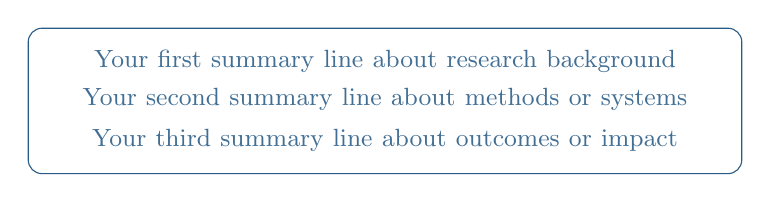
\begin{tikzpicture}
\node[
    draw=sjtuBlue,
    rounded corners=5pt,
    fill=white,
    opacity=0.9,
    inner sep=8pt,
    text width=8.5cm,
    align=center,
    text opacity=1
]{
    \small\textcolor{sjtuBlue!80}{
        \CoverLineOne\\[0.3em]
        \CoverLineTwo\\[0.3em]
        \CoverLineThree
    }
};
\end{tikzpicture}

\vspace{0.6em}
{\small
\faUniversity~\Affiliation\\[0.2em]
\faCalendar~\PresentationDate\\[0.2em]
}
\end{column}

\begin{column}{0.18\textwidth}
\end{column}
\end{columns}

\vfill
{\footnotesize\color{gray}
\faEnvelope~\Email \quad
\faPhone~\Phone \quad
\faGithub~\GitHub
}
\note{\scriptsize Cover page speaking notes: introduce yourself, greet the audience, state the topic. (1min)

\medskip\textbf{---中文---}\newline
封面页演讲稿：自我介绍、问候听众、引出主题。(1分钟)}
\end{frame}
\else
% --- Cover WITHOUT photo ---
\begin{frame}[plain]
\begin{tikzpicture}[remember picture,overlay]
    \node[anchor=center,inner sep=0pt] at (current page.center) {
        
\includegraphics[width=\paperwidth,height=\paperheight]{assets/封面.png}
    };
\end{tikzpicture}

\vspace{0.8cm}
\begin{center}

\includegraphics[width=4cm]{assets/校标-标志中英文横版.png}\\[0.3em]
{\LARGE\bfseries\textcolor{sjtuBlue}{\PresenterName}}\\[0.4em]
{\normalsize\color{gray}\PresentationSubtitle}\\[0.8em]

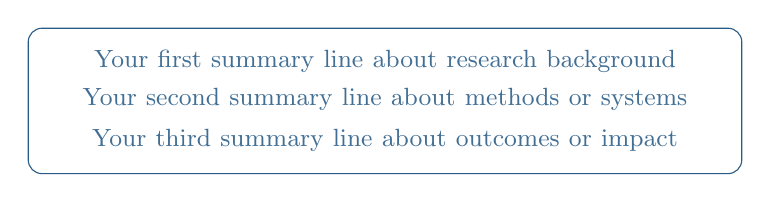
\begin{tikzpicture}
\node[
    draw=sjtuBlue,
    rounded corners=5pt,
    fill=white,
    opacity=0.9,
    inner sep=8pt,
    text width=8.5cm,
    align=center,
    text opacity=1
]{
    \small\textcolor{sjtuBlue!80}{
        \CoverLineOne\\[0.3em]
        \CoverLineTwo\\[0.3em]
        \CoverLineThree
    }
};
\end{tikzpicture}

\vspace{0.6em}
{\small
\faUniversity~\Affiliation\\[0.2em]
\faCalendar~\PresentationDate\\[0.2em]
}
\end{center}

\vfill
{\footnotesize\color{gray}
\faEnvelope~\Email \quad
\faPhone~\Phone \quad
\faGithub~\GitHub
}
\note{\scriptsize Cover page speaking notes: introduce yourself, greet the audience, state the topic. (1min)

\medskip\textbf{---中文---}\newline
封面页演讲稿：自我介绍、问候听众、引出主题。(1分钟)}
\end{frame}
\fi


% ==================== Layout A: Left Text + Right Figure ====================
% === EDIT: Duplicate this frame for each text+figure slide ===
\begin{frame}{Layout A: Left Text + Right Figure}
\begin{columns}[T,totalwidth=\textwidth]
\begin{column}{0.48\textwidth}

\begin{block}{Key Points}
\tagitem{Tag1} \tagitem{Tag2} \tagitem{Tag3}
\vspace{0.2em}
% === EDIT: Replace bullets ===
\begin{itemize}
    \item First core point with context.
    \item Second core point with technical detail.
    \item Third core point with implication.
\end{itemize}
\end{block}

\vspace{0.2em}
\begin{block}{Quantitative Outcome}
\begin{itemize}
    \item Main metric: \metric{+XX\%}
    \item Error reduction: \metric{-YY\%}
\end{itemize}
\end{block}

\end{column}

\begin{column}{0.49\textwidth}
\centering
% === EDIT: Replace figure path ===

\includegraphics[width=\textwidth]{figures/example_figure.png}

\vspace{0.3em}
{\scriptsize Figure caption here.}
\end{column}
\end{columns}
\note{\scriptsize Explain the key points shown on this slide and walk through the figure. (2min)

\medskip\textbf{---中文---}\newline
讲解本页要点，结合右侧图表进行说明。(2分钟)}
\end{frame}


% ==================== Layout B: Full-Width Content ====================
% === EDIT: Duplicate this frame for full-width slides ===
\begin{frame}{Layout B: Full-Width Content}

\begin{block}{Main Argument}
\begin{itemize}
    \item Background and motivation.
    \item Problem statement and constraints.
    \item Proposed approach and novelty.
\end{itemize}
\end{block}

\vspace{0.25em}
\begin{block}{Evidence}
\centering
\begin{tabular}{lcc}
\toprule
Item & Baseline & Proposed \\
\midrule
Metric A & 0.00 & 0.00 \\
Metric B & 0.00 & 0.00 \\
Metric C & 0.00 & 0.00 \\
\bottomrule
\end{tabular}

\vspace{0.3em}
{\scriptsize One-line interpretation of the table above.}
\end{block}

\note{\scriptsize Present the main argument and interpret the evidence table. (2min)

\medskip\textbf{---中文---}\newline
阐述核心论点，解读表格中的数据对比。(2分钟)}
\end{frame}


% ==================== Layout C: Two-Column Blocks ====================
% === EDIT: Duplicate this frame for two-column block slides ===
\begin{frame}{Layout C: Two-Column Blocks}
\begin{columns}[T,totalwidth=\textwidth]

\begin{column}{0.49\textwidth}
\begin{block}{Left Block Title}
\begin{itemize}
    \item Left-side argument 1.
    \item Left-side argument 2.
    \item Left-side argument 3.
\end{itemize}
\end{block}
\end{column}

\begin{column}{0.49\textwidth}
\begin{block}{Right Block Title}
\begin{itemize}
    \item Right-side argument 1.
    \item Right-side argument 2.
    \item Right-side argument 3.
\end{itemize}
\end{block}
\end{column}

\end{columns}
\note{\scriptsize Compare the two columns and highlight the key differences. (2min)

\medskip\textbf{---中文---}\newline
对比两列内容，强调关键差异。(2分钟)}
\end{frame}


% ==================== Thank You Page (Fixed Layout) ====================
\begin{frame}[plain]
\begin{tikzpicture}[remember picture,overlay]
    \node[anchor=center,inner sep=0pt] at (current page.center) {
        
\includegraphics[width=\paperwidth,height=\paperheight]{assets/封面.png}
    };
\end{tikzpicture}

\vspace{2.5cm}
\begin{center}
{\Huge\bfseries\textcolor{sjtuBlue}{Thank You}}\\[1em]
{\Large\color{gray}Questions and Discussion}\\[2em]

{\normalsize
\faEnvelope~\Email\\[0.3em]
\faPhone~\Phone\\[0.3em]
\faGithub~\GitHub
}
\end{center}
\note{\scriptsize Summarize the key takeaways, thank the audience, invite questions. (1min)

\medskip\textbf{---中文---}\newline
总结要点，感谢听众，欢迎提问。(1分钟)}
\end{frame}

\end{document}
